%% pdf 加密操作:
%\special{pdf:encrypt ownerpw (2436946) userpw () length 128 perm 2052} 
%///////////////////////////////////////////////////////////////////////////////
\documentclass[12pt,a4]{article} % or report
\usepackage{cx}
\usepackage{cx_ml}

\usepackage[open,openlevel=2,numbered]{bookmark}
% \pdfbookmark[section]{Contents}{toc} % 在生成的 pdf 书签中添加 “目录”


%% 设置全文脚注连续编号,latex默认每章重新清零编号。
\counterwithout*{footnote}{section}

%% 设置页边距:
\usepackage{geometry}
\geometry{left=3.5cm,right=3.5cm,top=1cm,bottom=2cm}


%% 行距、段距设置
%\linespread{1.2}     % 设置基本行距。
% article 文档类的默认是1,即1.2倍字号大小;
% ctexart 文档类的默认是1.3,即1.56倍字号大小。
\setlength\parskip{5pt}   % 段间距


%% 将默认的「标题」改为自定义内容
%\renewcommand{\contentsname}{My list of contents}
%\renewcommand{\listfigurename}{My list of figures}
%\renewcommand{\listtablename}{My list of table}
%\renewcommand{\bibname}{参考文献}
%\renewcommand{\figurename}{图}
%\renewcommand{\tablename}{表}


%% 另一种花体
%\usepackage{mathrsfs}   


\usepackage{caption,subcaption}       % 可以用 \caption*{} 不把图片或表格进行编号 

%% 生成封面图片, 参数 cc 表示垂直居中:
% \usepackage[cc]{titlepic}  


\usepackage{bm}            % 数学环境加粗字体

%% 各章前添加一个目录:
%\usepackage{titletoc}      



%% 边注
\usepackage[backgroundcolor=white,linecolor=magenta,textwidth=4em,textsize=footnotesize,disable]{todonotes}
%% \todo{here's a comment in the margin!}
%% \todo[inline, color=green!40]{This is an inline comment.}



%% 勾勾+叉叉
\usepackage{pifont}% http://ctan.org/pkg/pifont
\newcommand{\cmark}{\ding{51}}
\newcommand{\xmark}{\ding{55}}



\usepackage[numbers,sort&compress]{natbib}
\usepackage{quiver}


\newcommand{\dashto}{\dashrightarrow}
\newcommand{\vsim}{\;|\hspace{-1ex}\sim}

\usepackage{multirow}


% 附录中定理环境
\usepackage{chngcntr}
\usepackage{apptools}
\AtAppendix{\counterwithin{thm}{section}}


%//////////////////////////////////////////////////////////////////////////////
%% title page:
\title{ 
	Notes on Abstract Argumentation Theory
}
\author{
	\textsc{Xin Chen}  
	(\href{mailto:chenxin_hello@outlook.com}
	{\textsf{chenxin\_hello@outlook.com}})
}
\date{Latest edit: \today}


%///////////////////////////////////////////////////////////////////////////////
\begin{document}


\maketitle


This note gives a concise introduction to Dung's abstract argumentation theory \cite{Dun1995} and  some extensions (probabilistic extension, in particular).
% 
We mainly investigate Dung's original notions of \textit{complete}, \textit{grounded}, \textit{preferred}, and \textit{stable} semantics. 
However, 
for other semantics which are available in the literature since Ding's seminal work \cite{Dun1995}, 
for instance, 
\textit{semi--stable}, \textit{ideal}, \textit{eager}, \textit{stage}, \textit{CF2} and \textit{stage2} semantics \cite{Bar.Gia2009, Bar.Cam.Gia2018}, 
will be considered in the next version of this note.






% /////////////////////////////////////////////////////////////////////////////
\pdfbookmark[section]{Contents}{toc}
\tableofcontents
\section{Abstract Argumentation Theory}
\label{sec: AAT}



This section is devoted to the \textit{abstract argumentation theory} introduced in the seminal paper by  Dung \cite{Dun1995}.
% 
This formalism is based on the idea that arguments are defeasible entities which may attack each other and whose acceptance is subject to a given reasonable criterion (called \textit{semantics}).
% 
Formally, 
an argumentation framework is represented as a directed graph in which the arguments are represented as nodes and the attack relations as  edges.
% 


Given such a graph, 
a key question is which set(s) of arguments can be accepted.
That is, 
once the argumentation framework has been constructed, 
how to determine which arguments to accept or reject?
% 
To answer this kind of questions corresponding to define an \textit{argumentation semantics}.
%
% 
By and large, 
two kinds of approaches for argumentation semantics are available in the literature: 
\begin{enumerate}[itemsep=5pt,parsep=0pt,leftmargin=3em,topsep=5pt,label=(\arabic*)]
    \item the \textit{extension}-based approach (proposed in Dung's original paper \cite{Dun1995}), and
    \item the \textit{labelling}-based approach.
\end{enumerate}
% 
In this note, 
however, 
for the sake of simplicity,
we only focus on the first one.
% , let alone the correspondence between those two approaches.





% Dung's theory can be regarded as an attack/conflict calculus, 
% which has been initially formulated for the need of dealing with attacks between arguments but then stands on its own feet, 
% even independently of the original interpretation in argumentative terms.



% applications: 
% \begin{itemize}[itemsep=5pt,parsep=5pt,leftmargin=3em,topsep=5pt]
%     \item inference from a knowledge base
%     \item decision--making
%     \item coalition formation
%     \item stable marriage problem
%     \item argument-based reasoning
% \end{itemize}


% When an argumentation framework was given,
% it is then interesting to identify the \textit{conflict-free outcomes}, 
% which, roughly speaking, 
% means determining which arguments should be accepted (let's say, ``survive the conflict'') and which arguments should be rejected (let's say, ``are defeated in the conflict''), 
% according to some reasonable criterion.
% % 
% A formal method to identify those outcomes for any argumentation framework is called \textit{argumentation semantics}.
% 
% 



\begin{comment}

The idea underlying the \textit{labelling}-based approach is to give each argument a label. 
A sensible (though not the only possible) choice for the set of labels is $\Lambda = \{\mathsf{in}, \mathsf{out}, \mathsf{undec}\}$,
where the label \textsf{in} means the argument is accepted, 
the label \textsf{out} means the argument is rejected and the label \textsf{undec} means one abstains from an opinion on whether the argument is accepted or rejected. 
Each argument then gets exactly one label.

A specific labelling-based argumentation semantics provides a way to select “reasonable” labellings among all the possible ones, 
according to some criterion embedded in its definition.


A first investigation of the connections between defeat status assignments and extensions in Dung's argumentation frameworks was provided in \cite{Verheij1996}.

\dotfill
\vspace{1.5em}
\end{comment}








% Some preliminaries and notation: 
% arguments in any argumentation framework will be denoted by lowercase Latin letters: $a,b,c, \dots$.






% central notion: acceptability of arguments.





% \textit{The one who has the last word laughs best}.



% \vspace{3em}



% Roughly, 
% the idea of argumentational reasoning is that a statement is believable if it can be argued successfully against attacking arguments. 
% In other words, 
% whether or not a rational agent believes in a statement depends on whether or not the argument supporting this statement can be successfully defended against the counterarguments. 



% \vspace{3em}


%  argumentation  can be viewed as logic programming with negation as failure.
% % 
% This result shows that logic programming is the perfect tool for implementing argumentation systems.


% \vspace{3em}




% /////////////////////////////////////////////////////////////////////////////
\subsection{Argumentation frameworks}
\label{subsec: AFs}


An (abstract) argumentation framework is nothing, 
mathematically speaking, 
but a pair consists of a set of arguments and a binary relation representing the attack relationship between arguments, 
that is, 
a \textit{directed graph} in which the arguments as nodes and the attack relations as arrows. 
% 
An argument is an abstract entity whose role is solely determined by its relations to other arguments.



\begin{df}[Argumentation frameworks]
    An \textit{argumentation framework} (AF) is a pair 
    \[
        AF = (Ar,\to)
    \]
    where $Ar$ is a non-empty set of arguments, 
    and $\to$ is a binary relation on $Ar$, 
    i.e.,
    $\to\; \subseteq A \times A$.
\end{df}



Given an AF $AF=(Ar,\to)$, 
let $a,b \in Ar$, 
we say that $a$ \textit{attacks/defeats} $b$ (accordingly, $a$ is an \textit{attacker} of $b$) iff $a \to b$ holds.
% 
For any $X \cup \{a\} \subseteq Ar$, 
then we say that $X$ \textit{attacks} $a$, 
denoted as $X \to a$, 
if there exists $b \in X$ such that $b \to a$.
% 
Likewise, 
we say that $a$ \textit{attacks} $X$, 
written as $a \to X$, 
if there is $b \in X$ such that $a \to b$.
% 
% 
For $a \in Ar$, 
we define $a^-$ and $a^+$ as follows:
\[
\begin{array}{rll}
    a^- &\coloneqq& \{b \in Ar \mid b \to a\},  \\
    
    a^+ &\coloneqq& \{b \in Ar \mid a \to b\}.  \\
\end{array}
\]
Those two operations can be extended to any subset $X \subseteq Ar$ by
\[
    X^\circ   = \bigcup_{a \in X} a^\circ 
    \qquad
    \circ \in\{+,-\}.
\]





The attack relations between argument(s) aforementioned are summarized by Table~\ref{tab: attack-relation}. 
% In what follows, 
% we will use $\not\to$ to denote the negation of $\to$.



% attack relationships
\begin{table}[ht!]
    \centering
    \caption{The attack relations between argument(s)}
    \label{tab: attack-relation}
    % 
    \renewcommand{\arraystretch}{1.3}
    \begin{tabular}{l||ll}
    \hline
    \multicolumn{1}{c||}{notation} & 
    \multicolumn{1}{c}{meaning} \\
    \hline

    $a \to b$ & 
    $a$ attacks $b$  \\

    $a \to X$ &  
    $a$ attacks $X$ ($\exists b \in X: a \to b$) \\ 

    $X \to a$  &  
    $X$ attacks $a$  ($\exists b \in X: b \to a$) \\

    
    $X \to Y$ &
    $X$ attacks $Y$ 
    ($\exists a \in X, \exists b \in Y: a \to b$)  \\

    % $\dashrightarrow$  \\ 
    % $a \dashto b$ &  \\

    % $a \leadsto  b$  \\

    % $a \twoheadrightarrow  b$  \\
    \hline
\end{tabular}
\end{table}






% \begin{df}[Subframes]
%     Given an AF $\mathcal{AF} = (Ar,\to)$ and a set of arguments $X \subseteq Ar$, 
%     the restriction of $\mathcal{AF}$ to $X$, 
%     denoted as $\mathcal{AF}_X$, 
%     is the argumentation framework $(X,\to_X)$ where 
%     $\to_X \;=\; \to \cap (X\times X)$.    
% \end{df}








% \vspace{3em}
% Doing abstract argumentation theory means, essentially, 
% to study specific properties of subsets of the set of arguments in a given argumentation framework.




% \begin{df}[Conflict-freeness, Acceptability and Admissibility] 
%     Let $\mathcal{AF} = (A,\to)$ be an argumentation framework, and $X \subseteq A$:
%     \begin{enumerate}[itemsep=5pt,parsep=5pt,leftmargin=3em,topsep=5pt,label=(\arabic*)] %% or label = \alph*, \roman*
%         \item 
%         A set $X$ of arguments is said to be \todo{无冲突} {\color{purple} \textit{conflict-free}} if there are no arguments $a$ and $b$ in $X$ s.t. $a$ attacks $b$, 
%         formally, 
%         $\neg\exists a,b \in X: a \to b$. 

%         \item 
%         An argument $a$ is {\color{purple} \textit{acceptable}} w.r.t. a set $X$ of arguments iff for each argument $b$: 
%         if $b$ attacks $a$ then $b$ is attacked by $X$.

%         \item 
%         A conflict-free set of arguments $X$ is {\color{purple} \textit{admissible}} iff each argument in $X$ is acceptable w.r.t. $X$.
%     \end{enumerate}
% \end{df}










% /////////////////////////////////////////////////////////////////////////////
% \subsection{Argumentation Semantics (extension-based)}
% \subsection{Argumentation Semantics}
% \label{subsec: basic-definition}







% \vspace{1.5em}

% a simple principle: 
% for every argument $a$ one accepts or rejects one should be able to explain why it is accepted or rejected, 
% taking into account the acceptance or rejection of other arguments connected to $a$ through the attack relation. 




---


\begin{df}[Defense]
    Let $AF=(Ar,\to)$ be an AF and $X \subseteq Ar$. 
    % 
    The set $X$ \textit{defends} $a \in Ar$ 
    (or, $a$ \textit{acceptable} w.r.t. $X$) 
    iff 
    $\forall b \in Ar:b \to a \Rightarrow X \to b$
    (or equivalently, $\forall b \in a^- : X \to b$, 
    where $a^-$ is the set of attackers of $a$).
    \footnote{
        The original terminology in Dung's paper \cite{Dun1995} was that ``$a$ is \textit{acceptable} w.r.t. $X$''.
    }
\end{df}




According to vacuous truth,
if $a^- = \emptyset$
(such $a$ are called \textit{initial arguments}, 
the set of initial arguments of an AF $AF$ denoted as $\mathcal{NI}(AF)$, i.e., 
$\mathcal{IN}(AF) =  \{a \in Ar \mid a^- = \emptyset\}$)
then $a$ defended by any set of arguments, 
including $\emptyset$ of course.




\begin{df}[Characteristic function]
    Let $AF=(Ar,\to)$ be an AF. 
    % 
    The \textit{characteristic function} of $AF$ is mapping 
    $C_{AF} \colon \wp(Ar) \to \wp(Ar)$ such that 
    \[
        C_{AF} (X) 
            = 
        \{a \in Ar \mid X \text{~defends~} a\}
    \]
    for each $X \subseteq Ar$. 
\end{df}

% In what follows, 
% for the sake of brevity,
% we will simply notate $C_{AF}$ as $C$ if no confusion arises.


\begin{prop} 
    For any AF $AF=(Ar,\to)$, 
    then:
    \begin{enumerate}[itemsep=5pt,parsep=5pt,leftmargin=3em,topsep=5pt,label=(\arabic*)] %% or label = \alph*, \roman*
        \item $C_{AF}(\emptyset)=\mathcal{IN}(AF)=\{a \in Ar \mid a^- = \emptyset\}$.
        

        \item $\mathcal{IN}(AF) \subseteq C_{AF}(X)$.


        \item $C_{AF}(X) = (X^+)^+$.
        % [AC98] L. Amgoud and C. Cayrol. On the acceptability of arguments in preference-based argumentation. In G. Cooper and S. Moral, editors, Proceedings of the 14th Conference on Uncertainty in Artificial Intelligence (UAI 1998), pages 1–7. Morgan Kaufmann, 1998.
    \end{enumerate}
    where $X \subseteq Ar$.
\end{prop}




\begin{df}[Conflict-freeness]
    Let $AF=(Ar,\to)$ be an AF and $X \subseteq Ar$.
    % 
    $X$ is said to be  \textit{conflict-free} iff 
    $\neg\exists a,b \in X: a \to b$. 
\end{df}



Clearly, 
the emptyset $\emptyset$ is conflict--free.
%
Furthermore,  
if each argument has at least one attacker in an AF, 
i.e. $a^- \not=\emptyset$ for every argument $a$, 
then  $\emptyset$ is a (conflict--free) fixed point of the characteristic function.




After introduced the notion of \textit{defense}, 
a basic requirement for a set of arguments is the capability to defend all its elements. 
% 




\begin{df}[Admissibility]
    Let $AF=(Ar,\to)$ be an AF. 
    A set $X \subseteq Ar$ is called an \textit{admissible set} iff 
    (1) $X$ is conflict-free and 
    (2) $X \subseteq C_{AF}(X)$.
    % 
    % The set of admissible sets of $\mathcal{AF}$ is denoted as $AS_\mathcal{AF}$.
\end{df}


Thus, 
an admissible set is required to be both internally coherent, 
that is, conflict-free and able to defend its elements.
% 
Admissible sets always exist.
% 
A very trivial case is that the empty set $\emptyset$ is admissible for any argumentation framework.





\begin{example}
    \[AF: \qquad
    \begin{tikzcd}
        a & b & c & d
        \arrow[from=1-1, to=1-2]
        \arrow[from=1-2, to=1-3]
        \arrow[curve={height=-10pt}, from=1-3, to=1-4]
        \arrow[curve={height=-10pt}, from=1-4, to=1-3]
    \end{tikzcd}\]

    - non-empty conflict-free sets: 
    $
        \{a\}, 
        \{b\},
        \{c\},
        \{d\},
        \{a,c\},
        \{a,d\},
        \{b,d\}.
    $

    - non-empty admissible sets:
    $
        \{a\}, 
        \{d\},
        \{a,c\},
        \{a,d\}.
    $

    - $C_{AF}(\{a\}) = \{a\}$, 
    $C_{AF}(\{d\}) = \{d,a\}$, 
    $C_{AF}(\{a,c\}) = \{a,c\}$,
    $C_{AF}(\{a,d\}) = \{a,c,d\}$.
\end{example}



Finally, 
it is worth recalling that admissibility and defense are related by a basic property. 
In terms of extensions, 
if an admissible set defends an argument, 
it is possible to add the argument to the set while preserving its admissibility and its capability to defend any other argument. 
This was proved in the so-called Dung's Fundamental Lemma.


\begin{lemma}[Dung's Fundamental Lemma \cite{Dun1995}]
    For any AF $AF=(Ar,\to)$, 
    let $X$ be an admissible set and $a,b$ be arguments defended by $X$. 
    Then 
    \begin{enumerate}[itemsep=5pt,parsep=5pt,leftmargin=3em,topsep=5pt,label=(\arabic*)] %% or label = \alph*, \roman*
        \item $X'=X\cup\{a\}$ is an admissible set; 
        \item $X'$ defends $b$.
    \end{enumerate}   
\end{lemma}





% \begin{df}[Strong admissibility]
%     Let $(Ar,\to)$ be an AF, 
%     $X \subseteq Ar$ is \textit{strongly admissible} iff 
%     every $a \in X$ is defended by some $Y \subseteq X \setminus \{a\}$ which is strongly admissible.
% \end{df}

% In case there are no unattacked arguments in a framework, 
% the empty set is its only strongly admissible set.




\begin{comment}
% /////////////////////////////////////
\subsubsection{principle for extension-based semantics}

reasonable general properties which are shared by all (or, at least, most) existing semantics and can be regarded as evaluation principles for new ones.


\begin{enumerate}[itemsep=5pt,parsep=5pt,leftmargin=3em,topsep=5pt,label=(\arabic*)] %% or label = \alph*, \roman*
    \item 
    \textbf{conflict-free principle} (a extension is a set of arguments which ``can stand together'').


    \item 
    \textbf{admissibility principl}e  (an extension is a set of arguments which ``can stand on its own'', 
    namely is able to withstand the attacks it receives from other arguments by ``replying'' with other attacks.)


    \item 
    \textbf{reinstatement principle}:  if the attackers of an argument $a$ are in turn attacked by an extension $E$ one may assume that they have no effect on $a$: 
    then $a$ should be, in a sense, \textit{reinstated}, 
    therefore it should belong to $E$.


    \item 
    \textbf{language independence principle}: 
    the set of extensions only depends on the attack relation between arguments while it is totally independent of any property of arguments at the underlying language level. 
    argumentation frameworks which are isomorphic have the “same” (modulo the isomorphism) extensions.



    \item 
    \textbf{I-maximality principle}: 
    Let $\mathcal{E}$ be a set of extensions, 
    $\mathcal{E}$ is $I$-maximal iff $\forall E_1,E_2 \in \mathcal{E}: E_1 \subseteq E_2 \Rightarrow E_1 = E_2$.
    ----> relationships between extensions.

    \item 
    \textbf{directionality principle}: 
    an argument $a$ may affect another argument $b$ only if there is a directed path from $a$ to $b$.
\end{enumerate}






% /////////////////////////////////////
\subsubsection{justification state:}


The justification state of an argument $a$ can be conceived in terms of its extension membership. 
A basic classification encompasses only two possible states for an argument, 
namely \textit{justified} or \textit{not justified}.
n this respect, 
two alternative types of justification, 
namely \textit{skeptical} and \textit{credulous} can be considered.


\begin{df}[skeptical and credulous arguemnts]
    For any semantics $\sigma$ and AF $\mathcal{AF}$, 
    an argument $a$ is:
    \begin{itemize}[itemsep=5pt,parsep=5pt,leftmargin=3em,topsep=5pt]
        \item 
        \textit{skeptically justified} iff $\forall E \in \mathcal{E}_\sigma(\mathcal{AF}), a \in E$.
        

        \item 
        \textit{credulously justified} iff $\exists E \in \mathcal{E}_\sigma(\mathcal{AF}), a \in E$.
    \end{itemize}
\end{df}

Clearly the two notions coincide for \textit{unique-status} approaches, 
while, in general, 
skeptical justification $\subseteq$ credulous justification.




\begin{figure}[!ht]
    \centering
    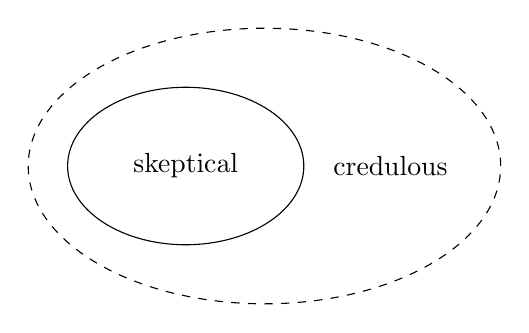
\begin{tikzpicture}
    \tikzstyle{every node}=[font=\normalsize]

    \draw[dashed]  (4,9.25) ellipse (3cm and 1.75cm);
    \draw  (3,9.25) ellipse (1.5cm and 1cm);
    \node [font=\normalsize] at (3,9.25) {skeptical};
    \node [font=\normalsize] at (5.6,9.25) {credulous};
    \end{tikzpicture}
\end{figure}





The following three justification states refine this relatively rough classification aforementioned:



\begin{df}[justified/defeasible/overruled arguemnts]
    Given a semantics $\sigma$ and an AF $\mathcal{AF}$, 
    an argument $a$ is: 
    \begin{itemize}[itemsep=5pt,parsep=5pt,leftmargin=3em,topsep=5pt]
        \item 
        \textit{justified} iff $\forall E \in \mathcal{E}_\sigma (\mathcal{AF}): a \in E$; 
        \hfill (= skeptical justification)
        

        \item 
        \textit{defensible} iff $\exists E_1,E_2 \in \mathcal{E}_\sigma (\mathcal{AF}): a \in E_1, a \not\in E_2$;


        \item 
        \textit{overruled} iff $\forall E \in \mathcal{E}_\sigma(\mathcal{AF}): a \not\in E$. 
        \hfill ($a$ should be rejected)
    \end{itemize}
\end{df}


\end{comment}


% /////////////////////////////////////////////////////////////////////////////
\subsection{An overview of (extension-based) argumentation semantics}


In this subsection we provide an overview of some well-known argumentation semantics, 
starting from the very basic notion of ``na\"{i}ve semantics'' \cite[\S~3.2]{Bar.Cam.Gia2018} and then 
discussing Dung's original concepts of \textit{complete}, \textit{stable}, \textit{preferred} and \textit{grounded} semantics \cite{Dun1995}.
% , 
% as well as the subsequently introduced \textit{ideal} [Dung et al., 2007], \textit{semi-stable} [Verheij, 1996; Caminada, 2006b] and \textit{eager} [Caminada, 2007b] semantics. 


% In this subsection, 
% we will examine several well-known extension-based argumentation semantics proposed in the literature. 
% 
% It is possible to distinguish between:
% \begin{itemize}[itemsep=5pt,parsep=5pt,leftmargin=2em,topsep=5pt]
%     \item four classical semantics stem from Dung's originally  seminal paper \cite{Dun1995}, 
%     namely (1) \textit{complete}, (2) \textit{grounded}, (3) \textit{stable} and (4) \textit{preferred} semantics;


%     \item 
%     subsequent proposals introduced by various authors in the literature, 
%     including \textit{stage}, \textit{semi-stable}, \textit{ideal}, $CF2$ and \textit{prudent} semantics, 
%     those semantics often overcome some limitation or improve some undesired behavior of Dung's original approach;

%     \item 
%     but in what follows, 
%     we start from a very na\"{i}ve one, 
%     called \textit{na\"{i}ve} semantics \cite[\S~3.2]{Bar.Cam.Gia2018}.
% \end{itemize} 




\begin{remark}
    In the literature, 
    \textit{admissibility} and \textit{conflict--freeness} mentioned in \S~\ref{subsec: AFs} are sometimes viewed as semantics, and sometimes as properties.
    We choose to treat them as properties in this note.
\end{remark}




\begin{df}[Extension-based semantics]
\label{def: extension-semantics}
    An \textit{extension-base semantics} (\textit{semantics}, for short) $\sigma$ associates with any argumentation framework $AF = (Ar,\to)$ is a subset of $\wp(Ar)$, 
    denoted as $\sigma(AF)$.    
    The elements in $\sigma(AF)$ are called \textit{extensions} (under semantics $\sigma$).


    Let $\mathcal{D}^\sigma$ be the class of AFs where a semantic $\sigma$ is defined, 
    that is, 
    \[
        \mathcal{D}^\sigma 
            = 
        \{AF \mid \sigma(AF)\not=\emptyset\}.
    \]
    % 
    A semantics $\sigma$ is called \textit{universally defined} if $\mathcal{D}^\sigma$ includes all AFs.
    % 
    If for all $AF \in \mathcal{D}^\sigma$ we have that $|\sigma(AF)| = 1$, 
    i.e. the semantics $\sigma$ always prescribes exactly one extension, 
    then $\sigma$ is said to belong to the \textit{unique-status approach}, 
    it is said to belong to the \textit{multiple-status approach}, 
    otherwise.
\end{df}



% /////////////////////////////////////
\subsubsection{Na\"{i}ve Semantics}


\textit{Na\"{i}ve semantics} (denoted as $\mathcal{N}\!\mathcal{A}$) corresponds to selecting as many arguments as possible, 
provided that there are no conflicts among them.  
% 
It is a sort of greedy strategy, 
driven by the only criterion of avoiding conflicts. 
% 
Formally it corresponds to requiring conflict--freeness together with a maximality property.




\begin{df}[Na\"{i}ve extensions]
    Let $(Ar,\to)$ be an AF. 
    % 
    A set $X \subseteq Ar$ is called a \textit{na\"{i}ve extension} iff 
    $X$ is a maximal conflict-free set.
\end{df}


\begin{example}
    \qquad

    \begin{center}
    \renewcommand{\arraystretch}{3}
    \begin{tabular}{c||c}
        \hline
        $AF$ & 
        na\"{i}ve  extensions $ \mathcal{N}\!\mathcal{A}(AF)$ \\ 
        \hline
    
    
        \begin{tikzcd}
            a & b & c & d
            \arrow[from=1-1, to=1-2]
            \arrow[from=1-2, to=1-3]
            \arrow[curve={height=-10pt}, from=1-3, to=1-4]
            \arrow[curve={height=-10pt}, from=1-4, to=1-3]
        \end{tikzcd} & 
        $\{ a,c \}, \{ a,d \}, \{b,d\}$  \\
    
        \hline 
    
        \begin{tikzcd}
            a & c \\
            b & d
            \arrow[from=1-1, to=1-2]
            \arrow[curve={height=-6pt}, from=1-1, to=2-1]
            \arrow[from=1-2, to=2-2]
            \arrow[curve={height=-6pt}, from=2-1, to=1-1]
            \arrow[from=2-1, to=1-2]
        \end{tikzcd}  &
        $\{a,d\}, \{b,d\},\{c\}$ \\
    
        \hline 
    
        \begin{tikzcd}
            a & b \\
            & c
            \arrow[curve={height=-6pt}, from=1-1, to=1-2]
            \arrow[curve={height=-6pt}, from=1-2, to=2-2]
            \arrow[curve={height=-12pt}, from=2-2, to=1-1]
        \end{tikzcd} & 
        $\{a\}, \{b\}, \{c\}$ \\
        \hline
    \end{tabular}
    \end{center}
\end{example}

  




% % /////////////////////////////////////
\subsubsection{Complete Semantics}

% $X$ 防御的所有论证都在 $X$ 中

\textit{Complete semantics} (denoted as $\mathcal{CO}$) can be regarded as a strengthening of the basic 
requirements enforced by the idea of admissibility, 
it lies at the heart of all Dung's semantics (see Fig.~\ref{fig: relations among extension notions}).


A complete extension is a conflict--free set which includes precisely those arguments it defends. 
That is, 
if an argument is defended by the set it should be in the set, 
and if an argument is not defended by the set, it should not be in the set.


\begin{df}[Complete extensions]
    Let $AF=(Ar,\to)$ be an AF. 
    %
    A set $X \subseteq Ar$ is called a \textit{complete extension} iff $X$ is conflict--free and $X = C_{AF}(X)$. 
\end{df}


Technically this means that a complete extension is a \textit{conflict--free fixed point} of the characteristic function.
% 
It is clear that every complete extension is an admissible set, 
but the reverse does not hold in general.
% 
% Intuitively, 
% the notion of complete extension captures the kind of confident relational agent who believe in every thing he can defend.



\begin{prop} Let $AF = (Ar,\to)$ be any AF.
    \begin{itemize}[itemsep=5pt,parsep=5pt,leftmargin=3em,topsep=5pt]
        \item $\mathcal{CO}(AF) \not= \emptyset$, 
        that is, 
        complete semantics is universally defined (see Definition~\ref{def: extension-semantics}).


        \item 
        $\emptyset \in \mathcal{CO}(AF)$ iff $\mathcal{NI}(AF) = \emptyset$, 
        where $\mathcal{NI}(AF) \coloneqq \{a \mid a^- = \emptyset\}$.

        
        \item 
        $\forall E \in \mathcal{CO}(AF): \mathcal{NI}(AF) \subseteq E$.
    \end{itemize}
\end{prop}






% complete extensions
\begin{example} \qquad

    \begin{center}
    \renewcommand{\arraystretch}{3}
    \begin{tabular}{c||c}
    \hline
        $\mathcal{AF}$ & 
        complete extensions $\mathcal{E}_\mathcal{CO}(\mathcal{AF})$ \\ 
        \hline
    
    
        \begin{tikzcd}
            a & b & c & d
            \arrow[from=1-1, to=1-2]
            \arrow[from=1-2, to=1-3]
            \arrow[curve={height=-10pt}, from=1-3, to=1-4]
            \arrow[curve={height=-10pt}, from=1-4, to=1-3]
        \end{tikzcd} & 
        $\{a\}, \{a,d\}, \{a,c\}$  \\
    
        \hline 
    
        \begin{tikzcd}
            a & c \\
            b & d
            \arrow[from=1-1, to=1-2]
            \arrow[curve={height=-6pt}, from=1-1, to=2-1]
            \arrow[from=1-2, to=2-2]
            \arrow[curve={height=-6pt}, from=2-1, to=1-1]
            \arrow[from=2-1, to=1-2]
        \end{tikzcd}  &
        $\emptyset, \{a,d\}, \{b,d\}$ \\
    
        \hline 
    
        \begin{tikzcd}
            a & b \\
            & c
            \arrow[curve={height=-6pt}, from=1-1, to=1-2]
            \arrow[curve={height=-6pt}, from=1-2, to=2-2]
            \arrow[curve={height=-12pt}, from=2-2, to=1-1]
        \end{tikzcd} & 
        $\emptyset$ \\
        \hline
    \end{tabular}
    \end{center}
\end{example}








% % /////////////////////////////////////
\subsubsection{Grounded Semantics}

% 满足怀疑的评价标准(最小的完全外延)

To accept only the arguments that one cannot avoid accepting, 
to reject only the arguments that one cannot avoid rejecting, 
and abstaining as much as possible.
% 
This gives rise to the most skeptical semantics among those based on complete extensions, 
namely the 
\textit{grounded semantics} (denoted as $\mathcal{GR}$).




\begin{df}[The grounded extension]
    Let $AF=(Ar,\to)$ be an AF.
    % 
    The \todo{基外延}\textit{grounded extension} of $AF$ is a minimal conflict--free fixed point of the characteristic function.
\end{df}


Notice that the uniqueness of the grounded extension. 
Since the characteristic function $C_{AF}$ is monotonic, 
it follows from the Knaster-Tarski Theorem that $C_{AF}$ has a unique smallest fixed point, 
it can then be proved that this fixed point is also conflict--free.



\begin{prop}
    For any AF $AF=(Ar,\to)$, 
    the following statements are equivalent:
    \begin{enumerate}[itemsep=5pt,parsep=5pt,leftmargin=3em,topsep=5pt,label=(\arabic*)] 
        \item $X$ is a minimal conflict--free fixed point of $C_{AF}$.
        
        \item $X$ is the smallest fixed point of $C_{AF}$.
    \end{enumerate} 
\end{prop}



It follows that:
\begin{itemize}[itemsep=5pt,parsep=5pt,leftmargin=3em,topsep=5pt]
    \item the grounded extension is unique 
    (i.e. grounded semantics belongs to the unique-status approach);


    \item the grounded extension is the least complete extension, 
    in particular it is included in any complete extension.
\end{itemize}




The grounded extension of an argumentation framework $AF$ will be denoted as $GR(AF)$.
% 
By definition,
the grounded extension coincides with the intersection of all complete extensions, 
that is 
\[
    GR(AF) = \bigcap \mathcal{CO} (AF).
\]
Hence, 
a unique grounded extension always exists, 
although it may be the empty set. 
% 
% It contains all the arguments which are not defeated, 
% as well as the arguments which are defended directly or indirectly by non-defeated arguments.



\begin{prop}
    If there are no initial arguments in an AF, 
    then the grounded extension is the empty set. 
    % 
    That is, 
    $\mathcal{IN}(AF) = \emptyset \Rightarrow GR(AF)=\emptyset$.
\end{prop}


\begin{example}[Grounded extension] \qquad

    \begin{center}
    \renewcommand{\arraystretch}{3}
    \begin{tabular}{c||c}
    \hline
        $AF$ & 
        grounded extensions $\mathcal{GR}(AF)$ \\ 
        \hline
    
    
        \begin{tikzcd}
            a & b & c & d
            \arrow[from=1-1, to=1-2]
            \arrow[from=1-2, to=1-3]
            \arrow[curve={height=-10pt}, from=1-3, to=1-4]
            \arrow[curve={height=-10pt}, from=1-4, to=1-3]
        \end{tikzcd} & 
        $\{a\}$  \\
    
        \hline 
    
        \begin{tikzcd}
            a & c \\
            b & d
            \arrow[from=1-1, to=1-2]
            \arrow[curve={height=-6pt}, from=1-1, to=2-1]
            \arrow[from=1-2, to=2-2]
            \arrow[curve={height=-6pt}, from=2-1, to=1-1]
            \arrow[from=2-1, to=1-2]
        \end{tikzcd}  &
        $\emptyset$ \\
    
        \hline 
    
        \begin{tikzcd}
            a & b \\
            & c
            \arrow[curve={height=-6pt}, from=1-1, to=1-2]
            \arrow[curve={height=-6pt}, from=1-2, to=2-2]
            \arrow[curve={height=-12pt}, from=2-2, to=1-1]
        \end{tikzcd} & 
        $\emptyset$ \\
        \hline
    \end{tabular}
    \end{center}
\end{example}




% % /////////////////////////////////////
\subsubsection{Preferred Semantics}

% 满足轻信的评价标准(极大的完全外延)

The idea of maximizing accepted arguments is expressed by \textit{preferred semantics} ($\mathcal{PR}$).


\begin{df}[Preferred extensions]
    Let $AF=(Ar,\to)$ be an AF. 
    %
    A \todo{优先外延} \textit{preferred extension} is a maximal (w.r.t. $\subseteq$) admissible set of $AF$. 
\end{df}



Every argumentation framework possesses at least one preferred extension.
Hence, 
preferred extension semantics is always defined for any argumentation framework. 
% 
Relationships of preferred extensions with other semantics notions have been analyzed in Dung's \cite{Dun1995}. 
%
Preferred extensions can for instance equivalently be characterized as maximal complete extensions.


\begin{prop}
    Let $AF=(Ar,\to)$ be an AF and $X \subseteq Ar$. 
    The following two statements are equivalent:
    \begin{enumerate}[itemsep=5pt,parsep=5pt,leftmargin=3em,topsep=5pt,label=(\arabic*)] 
        \item $X$ is a maximal admissible set of $AF$.
        
        \item $X$ is a maximal complete extension of $AF$.
    \end{enumerate}
\end{prop}


This in particular implies that the grounded extension is included in any preferred extension, 
as it is in any complete extension.


Preferred semantics has often been regarded as the most satisfactory semantics in the context of Dung's framework.



\begin{example}[Preferred extensions] \qquad

    \begin{center}
    \renewcommand{\arraystretch}{3}
    \begin{tabular}{c||c}
    \hline
        $AF$ & 
        preferred extensions $\mathcal{PR}(AF)$ \\ 
        \hline
    
        \begin{tikzcd}
            a & b & c & d
            \arrow[from=1-1, to=1-2]
            \arrow[from=1-2, to=1-3]
            \arrow[curve={height=-10pt}, from=1-3, to=1-4]
            \arrow[curve={height=-10pt}, from=1-4, to=1-3]
        \end{tikzcd} & 
        $\{a,d\}, \{a,c\}$  \\
    
        \hline 
    
        \begin{tikzcd}
            a & c \\
            b & d
            \arrow[from=1-1, to=1-2]
            \arrow[curve={height=-6pt}, from=1-1, to=2-1]
            \arrow[from=1-2, to=2-2]
            \arrow[curve={height=-6pt}, from=2-1, to=1-1]
            \arrow[from=2-1, to=1-2]
        \end{tikzcd}  &
        $\{a,d\}, \{b,d\}$ \\
    
        \hline 
    
        \begin{tikzcd}
            a & b \\
            & c
            \arrow[curve={height=-6pt}, from=1-1, to=1-2]
            \arrow[curve={height=-6pt}, from=1-2, to=2-2]
            \arrow[curve={height=-12pt}, from=2-2, to=1-1]
        \end{tikzcd} & 
        $\emptyset$ \\
        \hline
    \end{tabular}
    \end{center}
\end{example}




% % /////////////////////////////////////
\subsubsection{Stable Semantics}


\textit{Stable semantics} (denoted as $\mathcal{ST}$) relies on a very simple intuition: 
an extension should be able to attack all arguments not included in it.


\begin{df}[Stable extensions]
    Let $AF=(Ar,\to)$ be an AF. 
    %
    A \todo{稳定外延} \textit{stable extension} of $AF$ is a conflict--free set $X$ such that $X \cup X^+ = Ar$. 
\end{df}


A stable extension is an admissible set.
% 
In the context of game theory, 
the notion of stable extension coincides with the notion of \textit{stable solution} of $n$-person games \cite{Dun1995}. 
% 
Every stable extension is a preferred extension, 
but not vice versa. 


\begin{prop}
    Let $AF=(Ar,\to)$ be an AF and $X \subseteq Ar$. 
    The following statements are equivalent:
    \begin{enumerate}[itemsep=5pt,parsep=5pt,leftmargin=3em,topsep=5pt,label=(\arabic*)] 
        \item $X$ is a stable extension. 
        
        \item $X$ is an admissible set s.t. $X \cup X^+ = Ar$.
        
        \item $X$ is a complete extension s.t. $X \cup X^+ = Ar$.
        
        \item $X$ is a preferred extension s.t. $X \cup X^+ = Ar$.
        
        \item $X^+ = Ar \setminus X$.
    \end{enumerate}
\end{prop}


No stable extension is empty, 
and not every argument framework has stable extensions.



\begin{example}[Stable extensions] \qquad

    \begin{center}
    \renewcommand{\arraystretch}{3}
    \begin{tabular}{c||c}
    \hline
        $AF$ & 
        stable extensions $\mathcal{ST}(AF)$ \\ 
        \hline
    
    
        \begin{tikzcd}
            a & b & c & d
            \arrow[from=1-1, to=1-2]
            \arrow[from=1-2, to=1-3]
            \arrow[curve={height=-10pt}, from=1-3, to=1-4]
            \arrow[curve={height=-10pt}, from=1-4, to=1-3]
        \end{tikzcd} & 
        $\{a,d\}, \{a,c\}$  \\
    
        \hline 
    
        \begin{tikzcd}
            a & c \\
            b & d
            \arrow[from=1-1, to=1-2]
            \arrow[curve={height=-6pt}, from=1-1, to=2-1]
            \arrow[from=1-2, to=2-2]
            \arrow[curve={height=-6pt}, from=2-1, to=1-1]
            \arrow[from=2-1, to=1-2]
        \end{tikzcd}  &
        $\{a,d\}, \{b,d\}$ \\
    
        \hline 
    
        \begin{tikzcd}
            a & b \\
            & c
            \arrow[curve={height=-6pt}, from=1-1, to=1-2]
            \arrow[curve={height=-6pt}, from=1-2, to=2-2]
            \arrow[curve={height=-12pt}, from=2-2, to=1-1]
        \end{tikzcd} & 
        $-$ \\
        \hline
    \end{tabular}
\end{center}
\end{example}



% % /////////////////////////////////////


% \subsubsection{Semi-Stable Semantics}


% \textit{Semi-stable semantics} ($\mathcal{SST}$) 


% \begin{df}[Semi-stable extensions]
%     Let $\mathcal{AF}=(Ar,\to)$ be an AF. 
%     A \textit{semi--stable extension} of $\mathcal{AF}$ is a complete extension $X$ where $X \cup X^+$ is maximal among all complete extensions. 
% \end{df}


% % /////////////////////////////////////
% \subsubsection{Ideal and Eager Semantics}

% % /////////////////////////////////////
% \subsubsection{Stage Semantics}

% % /////////////////////////////////////
% \subsubsection{$CF2$ and stage2 Semantics}




% /////////////////////////////////////////////////////////////////////////////
\subsection{Computational problems and Complexity}



Given an AF $AF=(Ar,\to)$ and a semantics $\sigma$, 
the \textit{verification problem}, 
denoted as $Var_\sigma$, 
is deciding whether a set $X \subseteq Ar$ is a $\sigma$-extension of $AF$. 







For $a \in Ar$, 
the \textit{credulous acceptance problem}, 
denoted as $CA_\sigma$, 
is deciding whether $a$ is credulously accepted, 
that is deciding whether $a$ belongs to a $\sigma$--extension of $AF$.  
% 
Moreover, 
the \textit{skeptical acceptance problem}, 
denoted as $SA_\sigma$, 
is deciding whether $a$ is skeptically  accepted, 
that is deciding whether $a$ belongs to every $\sigma$--extension of $AF$. 

Clearly, 
$CA_\mathcal{GR}$ and $SA_\mathcal{GR}$
% that is $\sigma = \mathcal{GR}$, 
are identical problems.
% 
The computational complexity of those problems are summarized in  table~\ref{tab: complexity} \cite{Dun.Woo2009,Dvo.Dun2018}.


\begin{table}[ht!]
    \centering
    \caption{Complexity of $Ver$, $CA$ and $SA$ problems}
    \label{tab: complexity}
    %%
    \renewcommand{\arraystretch}{1.5}
    \begin{tabular}{c||ccc}
    \hline

    semantics & $Ver_\sigma$ & $CA_\sigma$ & $SA_\sigma$   \\
    \hline

    $\mathcal{CO}$ & 
    in P & 
    NP--c & 
    P--c  \\

    $\mathcal{GR}$ & 
    in P & 
    in P & 
    in P  \\

    $\mathcal{PR}$ & 
    coNP--c & 
    NP--c & 
    $\prod^p_2$--c  \\

    $\mathcal{ST}$ & 
    in P & 
    NP--c & 
    coNP--c  \\
    
    % semi-stable
    % $\mathcal{SS}$ & 
    % coNP--c & 
    % $\sum^p_2$--c & 
    % $\prod^p_2$--c  \\
    \hline
\end{tabular}
\end{table}





% \vspace{3em}
% One of the most common reasoning problems in argumentation concerns the skeptical and credulous acceptance of arguments, 
% by which we understand that they are accepted in all (resp. some) extensions of a given framework.

% $AF \vsim^c_\sigma a$ credulously accepted

% $AF \vsim^s_\sigma a$ skeptically accepted

% $AF \vsim^\circ_\sigma a$  where $\circ \in \{s,c\}$

% Every argument that does not attack itself will be credulously accepted under the conflict-free semantics.


% /////////////////////////////////////////////////////////////////////////////
\newpage
\newgeometry{left=.5cm,right=.5cm,top=1cm,bottom=2cm}
\subsection{A summary}


% The grounded extension is uniquely determined and always exists \cite{Dun1995}  and that not every framework is guaranteed to produce a stable extension.


\begin{table}[ht!]
    \centering
    \caption{Basic notions of AAT}
    \label{tab: basic notions of AAT}
    $AF = (Ar,\to)$ is an AF, $X \subseteq Ar$ and $a,b \in Ar$.
    \vspace{1em}

    \renewcommand{\arraystretch}{1.3}
    \begin{tabular}{l||lll}
    % Let $\mathcal{A} = (A,\to)$ be an abstract argumentation framework \\
    \hline
    \multicolumn{1}{c}{Notions}  & 
    \multicolumn{1}{c}{Definition or equivalent descriptions} \\
    \hline

    $a \to b$   &
    $a$ attacks/defeats $b$ \hfill  ($a$ is an attacker/counterargument of $b$)   \\

    $X \to a$ \qquad  ($X$ attacks $a$) & 
    $\exists b \in X: b \to a$  \\

    
    
    $a^-$ &  
    $a^- = \{b \in Ar \mid b \to a\}$  \\

    $a^+$ &  
    $a^+ = \{b \in Ar \mid a \to b\}$  \\

    $X^-$ &  
    $X^- = \{b \mid \exists a \in X: b \to a\} = \bigcup_{a\in X} a^- $\\

    $X^+$ & 
    $X^+ = \{b \mid \exists a \in X: a \to b\} = \bigcup_{a\in X} a^+$ \\


    $X$ defends $a$  / $a$ is admissible w.r.t. $X$ & 
    $\forall b: b \to a \Rightarrow X \to b$ 
    \hfill
    [$X$ defends $a$ for any $X$ if $a^- = \emptyset$]  \\

    
    $\mathcal{IN}(AF)$  &
    $\mathcal{IN}(AF) = \{a\in Ar \mid a^- = \emptyset\}$  
    \hfill  the set of initial arguments   \\

    \hdashline

    \multirow{3}*{
    $C_{AF}$: the characteristic function}  
    & 
    % $C_\mathcal{AF} \colon \wp(Ar) \to \wp(Ar)$ s.t. 
    $C_{AF} (X) = \{a \mid X \text{~defends~} a \}$   \\
    &  $C_{AF}{X} = (X^+)^+$  \\
    & [$\emptyset$ is a fixed point if $\mathcal{IN}(AF)=\emptyset$]  \\

    \hdashline


    $X$ is conflict--free & 
    $\not\exists a,b \in X: a \to b$ 
    \hfill
    [$\emptyset$ is conflict--free]  \\
    & 
    $\not\exists a,b \in X: a \in b^-$  \\ 
    & 
    $X \cap X^+ = \emptyset$    \\
    % $\forall a,b \in X: a \not\to b$  \\


    \hdashline


    $X$ is admissible & 
    $X$ is conflict--free and $X \subseteq C_\mathcal{AF} (X)$  
    \hfill
    [$\emptyset$ is admissible] \\

    
    \hline
    \multicolumn{2}{c}{Semantics} \\
    \hline

    $\mathcal{N}\!\mathcal{A}(AF)$:
    $X$ is a \textit{na\"{i}ve extension} & 
    $X$ is a maximal conflict--free set  \\
    \hdashline 


    $\mathcal{CO}(AF)$:
    $X$ is a \textit{complete extension} &  
    $X$ is a conflict--free  and $C_{AF}(X)=X$ 
    \quad
    (conflict--free fixed point) \\
    \hdashline


    \multirow{3}{*}{$\mathcal{GR}(AF)$:
    $X$ is the \textit{grounded extension} 
    } & 
    $X$ is the least fixed point of $C_{AF}$  \\
    & $X$ is the minimal complete extension  \\
    & $X = GR(AF) = \bigcap \mathcal{CO}(AF)$  \\
    \hdashline

    
    \multirow{2}{*}{$\mathcal{PR}(AF)$:
    $X$ is a \textit{preferred extension}  
    } & 
    $X$ is a maximal admissible set  \\
    & $X$ is a maximal complete extension  \\ 
    \hdashline

    
    \multirow{7}{*}{$\mathcal{ST}(AF)$: 
    $X$ is a \textit{stable extension}
    } & 
    $X$ is conflict--free and $X \cup X^+ = Ar$  \\
    & $X^+ = Ar \setminus X$    \\
    & $X$ is a preferred extension and $X \cup X^+ = Ar$  \\
    & $X$ is a complete extension and $X \cup X^+ = Ar$  \\
    & $X$ is admissible and $X \cup X^+ = Ar$  \\ 
    & $X = \{a \in Ar \mid X \not\to a\}$  \\
    & $X$ is conflict--free and attacks each argument that is not in $X$  \\
    \hline
    \end{tabular}

    % \vspace{1em}
    % NB: all the key argumentation-theoretic notions can be defined in terms of the characteristic function.
\end{table}


% It is well--known that
% the set of complete extensions forms a \textit{complete semilattice} w.r.t. $\subseteq$, 
% where $GR(AF)$ is the meet element, 
% whereas the greatest elements are the preferred extensions.



% % figure
\begin{figure}[ht!]
    \centering
    \begin{tikzcd}
	& {\text{stable~extension}} \\
	& \text{preferred~extension} \\
	\text{grounded~extension} & \text{complete~extension} & \text{na\"{i}ve~extension} \\
	& \text{admissible} \\
	& \text{conflict-free}
	\arrow[from=1-2, to=2-2]
	\arrow[curve={height=-12pt}, from=1-2, to=3-3]
	\arrow[from=2-2, to=3-2]
	\arrow[from=3-1, to=3-2]
	\arrow[from=3-2, to=4-2]
	\arrow[curve={height=-12pt}, from=3-3, to=5-2]
	\arrow[from=4-2, to=5-2]
    \end{tikzcd}
\caption{Relations among extension--based semantics}
\label{fig: relations among extension notions}
% \vspace{1em}
% \parbox{10cm}{\footnotesize
% Note: The intuitive meaning of  arrow ``$x \longrightarrow y$'' is that  ``every $x$ is a $y$'', 
% while the dashed arrow ``$x \dashrightarrow y$'' means that ``every $x$ is contained in any $y$''. 
% For example, 
% every stable extension is a preferred extension, 
% as well as, 
% the grounded extension is included in any preferred extensions.
% }
\end{figure}


\begin{table}[ht!]
    \centering
    \caption{A summary of the examples mentioned}
    \label{tab: example}
    \renewcommand{\arraystretch}{1.5}
    \begin{tabular}{c||ccccc}
    \hline
    AF & 
    na\"{i}ve  &
    complete & 
    grounded & 
    preferred & 
    stable \\
    \hline

    
    $\begin{tikzcd}
        a & b & c & d
        \arrow[from=1-1, to=1-2]
        \arrow[from=1-2, to=1-3]
        \arrow[curve={height=-10pt}, from=1-3, to=1-4]
        \arrow[curve={height=-10pt}, from=1-4, to=1-3]
    \end{tikzcd}$  & 
    $\begin{matrix} 
        \{a,c\}  \\
        \{a,d\}  \\
        \{b,d\}
    \end{matrix}$ & 
    $\begin{matrix} 
        \{a\}  \\
        \{a,c\}  \\
        \{a,d\}  
    \end{matrix}$  & 
    $\{a\}$  & 
    $\begin{matrix}
        \{a,c\} \\
        \{a,d\} 
    \end{matrix}$  & 
    $\begin{matrix}
        \{a,c\} \\
        \{a,d\} 
    \end{matrix}$  \\    
    [4ex]
    \hline 



    \begin{tikzcd}
        a & c \\
        b & d
        \arrow[from=1-1, to=1-2]
        \arrow[curve={height=-6pt}, from=1-1, to=2-1]
        \arrow[from=1-2, to=2-2]
        \arrow[curve={height=-6pt}, from=2-1, to=1-1]
        \arrow[from=2-1, to=1-2]
    \end{tikzcd} &  
    $\begin{matrix}
        \{a,d\} \\
        \{b,d\} \\
        \{c\}
    \end{matrix}$   & 
    $\begin{matrix}
        \emptyset \\
        \{a,d\} \\
        \{b,d\}
    \end{matrix}$  & 
    $\emptyset$   &  
    $\begin{matrix}
        \{a,d\} \\
        \{b,d\} 
    \end{matrix}$  &
    $\begin{matrix}
        \{a,d\} \\
        \{b,d\}
    \end{matrix}$  \\
    [4ex]
    \hline
   


    \begin{tikzcd}
        a & b \\
        & c
        \arrow[curve={height=-6pt}, from=1-1, to=1-2]
        \arrow[curve={height=-6pt}, from=1-2, to=2-2]
        \arrow[curve={height=-12pt}, from=2-2, to=1-1]
    \end{tikzcd} & 
    $\begin{matrix}
        \{a\} \\
        \{b\} \\
        \{c\}
    \end{matrix}$  & 
    $\emptyset$  & 
    $\emptyset$  & 
    $\emptyset$  & 
    $-$  \\
    [4ex]
    \hline
\end{tabular}
\end{table}


\restoregeometry
\newpage
% /////////////////////////////////////////////////////////////////////////////









% \section{Some extensions}
%///////////////////////////////////////


\cite{ArgAI2009}

% /////////////////////////////////////////////////////////////////////////////
\subsection{Preference--based AF}



Several works generalizing Dung's framework to handle preferences over arguments have been proposed. 
% (Amgoud and Cayrol 1998, 2002; Amgoud and Vesic 2011, 2014; Cyras 2016; Silva, Sa ́, and Alcaˆntara 2020).



\begin{df}[Preference--based Argumentation Frameworks, PAFs]
    A \textit{preference--based argumentation framework} (PAF) is a triple {\color{purple} $(Arg,\att,>)$} such that $(Arg,\att)$ is an AF and $>$ is a strict partial order  (i.e. an irreflexive, asymmetric and transitive relation) on $Arg$, 
    called \textit{preference relation}.    
\end{df}



For any $a,b \in Arg$, 
$a > b$ means that ``$a$ is better than $b$'' for the agent. 



The preference in a PAF $(Arg,\att,>)$ working as follows: 
classical argumentation semantics are used to obtain the extensions of the underlying $(Arg,\att)$, 
and then the preference relation $>$ is used to obtain a preference relation $\sqsupseteq$ over such extensions, 
so that the \textit{best extensions} w.r.t. $\sqsupseteq$ are eventually selected.


% There have been different proposals to determine the best extensions, 
% corresponding to different criteria to define $\sqsupseteq$ as explained in the following definition.




% /////////////////////////////////////////////////////////////////////////////
\subsection{Value--based AF}


The motivation behind VAFs (value--based argumentation frameworks) is to offer an explanatory mechanism accounting for choices between distinct justifiable collections $S$ and $T$, 
which are not collectively acceptable, 
i.e., $S$ and $T$ may be admissible under Dung's semantics, 
however, $S \cup T$ fails to be. 






%///////////////////////////////////////////////
\subsection{Probabilistic AF}

Recently, 
there are has been an increasing interest in modeling uncertainty in argumentation. 
% 
This has been carried out by combining probability theory with formal argumentation.
% 
The extension of Dung's abstract argumentation framework with probability theory is called \textit{probabilistic argumentation framework}.




In general a probabilistic argumentation framework consists of probabilistic arguments and probabilistic attacks \cite{Li.Ore.Nor2011,Faz.Fle.Par2015}.
% 
As shown in \cite{Man.Bis2020}, 
however, 
an argumentation framework with probabilities on both arguments and attacks can be transformed into an equivalent one with certain attack relations (i.e. the probability of each attack is $1$).\footnote{
    The equivalent transformation between those two kinds of probabilistic AFs has linear complexity \cite{Man.Bis2020}.
}
Hence, 
for the sake of brevity, 
in the section we only focus on probabilistic argumentation frameworks where only arguments are uncertain.



% \begin{df}[PrAFs \cite{Li.Ore.Nor2012}]
%     A \textit{probabilistic argumentation framework} (PrAF) is a tuple 
%     \[
%         (Ar,\to,p,p^\to)
%     \]
%     where $(Ar,\to)$ is an AF, 
%     $p$ and $p^\to$ are, respectively, 
%     functions assigning a non-zero probability value to each argument in $Ar$ and attack in $\to$, 
%     that is,
%     $p \colon Ar \to (0,1] \cap \mathbb{Q}$ and 
%     $p^\to\!: \to \; \to (0,1] \cap \mathbb{Q}$.
% \end{df}


\begin{df}[Probabilistic Argumentation Frameworks, PrAFs]
    A \textit{probabilistic argumentation framework} (PrAF) is a tuple 
    \[
        {\color{purple} PAF = (Arg,\att,P)}
    \]
    where $(Arg,\att)$ is an argumentation framework and
    $P$ is a function assigning a non-zero probability value to each argument in $Arg$,
    that is,
    $P \colon Arg \to (0,1]$ 
    (or $P \colon Arg \to (0,1] \cap \mathbb{Q}$ to facilitate the calculation). 
\end{df}



% \begin{remark}
%     In some literature, 
%     for instance ,

%     the probability function is just $p \colon Ar \to (0,1]$.
% \end{remark}



Intuitively, 
the value assigned by $P$ to an argument $a$ represents the probability that $a$ actually occurs, 
% whereas the value assigned by $p^\to$ to a defeat $\langle a,b \rangle$ represents the conditional probability that $a$ defeats $b$ given that both $a$ and $b$ occur.
moreover, 
every attack $a \att b$ occurs with conditional probability 1, 
that is, 
$a$ attacks $b$ whenever both $a$ and $b$ occur.
% 
Or in a \textit{justification perspective}:
$P(a)$ is treated as the probability that $a$ is a justified point and therefore should appear in the graph, 
and $1-P(a)$ is the probability that $a$ is not a justified point and so should not appear in the graph.

Thus, 
an argument $a \in Arg$ is viewed as a probabilistic event which is independent from the other events associated with other arguments 
$a \not=b \in Arg$.

\vspace{1.5em}






The meaning of a PrAF is given in terms of \textit{possible worlds}. 
Given a PrAF $PAF=(Arg,\att,P)$, 
a \textit{possible world} of $PAF$ is an AF $(Arg',\att')$ which is the restriction of $(Arg,\att)$ to $Arg'$, 
that is, 
$Arg' \subseteq Arg$ and $\att' \;=\; \att \cap\; (Arg'\times Arg')$. 
% 
The set of all possible worlds of $PAF$ is denoted as {\color{purple} $pw(PAF)$}.



% \begin{df}[Subgraph]
% \label{def: subgraph}
%     For any given PrAF $\mathcal{PF}=(Ar,\to,p)$,     
%     an AF $G = (Ar',\to')$ is a \textit{subgraph} $G$ of $\mathcal{PF}$,  $G \sqsubseteq \mathcal{PF}$ in symbol, 
%     if $G$ is the restriction of the underlying AF $(Ar,\to)$ to $Ar'$, 
%     i.e., 
%     $Ar' \subseteq Ar$ and $\to' \;= (Ar'\times Ar')\; \cap \to$. 
%     % 
%     The set of all subgraphs of $\mathcal{PF}$ is denoted as $\mathsf{sub}(\mathcal{PF})$.
% \end{df}


% \begin{remark}
%     \textit{possible world}  



%     In literature, 
%     the \textit{subgraph} in Def.~\ref{def: subgraph} is also called a \textit{full subgraph} \cite{Hun2013,Dod.Wol2014}.
%     % 
%     Obviously, 
%     every $Ar' \subseteq Ar$ induces a unique (full) subgraph, 
%     and the number of subgraphs is equals to $|\wp(Ar)| - 1$.
% \end{remark}




The probability distribution over arguments can generate a probability distribution over  possible worlds (subgraphs) of the original argument framework. 
% 
Using the subgraphs, 
we can then explore the notions of probability distributions over admissible sets, extensions, and inferences.




The intuition hereby is as follows: 
for $a \in Arg$, 
$P(a)$ is the probability that $a$ belongs to an arbitrary possible world (full subgraph) of $PAF$; 
while $1-P(a)$ is the probability that $a$ does not exist in an arbitrary possible world (full subgraph). 


(using the justification perspective \cite{Hun2012}, 
where $P(a)$ means the probability that $a$ is justified in appearing in the graph) 



\vspace{1.5em}


We can use the probability assigned to each argument to generate a probability distribution over the subgraphs. 
So each subgraph can be viewed as an ``interpretation'' of what the argument graph should be. 
If all the arguments have probability $1$, 
then the argument graph itself has probability $1$, 
and that is the only interpretation we should consider (using the constellations approach). 
But, if one or more arguments has a probability less than $1$, 
then there will be multiple ``interpretations''. 
% 
So for instance, 
if there is exactly one argument $a$ in the framework $G$ with probability less than $1$, 
then there are two “interpretations”, 
the first with $a$, 
and the second without $a$. 
% 
So using the justification perspective, 
with the constellations approach, 
we can treat the set of subgraphs of a $G$ as a \textit{sample space}, 
where one of the subgraphs is the ``true'' argument graph.


\vspace{1.5em}




\begin{df}
    The \textit{interpretation} for a PrAF $PAF=(Arg,\att,P)$ is  function 
    % {\color{purple} probability distribution function} 
    $I$ over the set $pw(PAF)$ such that 
    each $w \in pw(PAF)$ is assigned by $I$ the probability 
    \[
        I(w) = \left( \prod_{a\in Arg(w)} P(a) \right) 
        \cdot
        \left( \prod_{a \in Arg \setminus Arg(w)} (1 - P(a)) \right)
    \]
    where $Arg(w)$ is the set of arguments in $w$.
\end{df}


Thus, 
the probability of a subgraph captures the degree of certainty that the subgraph contains exactly the arguments that are regarded as holding.


\begin{thm}[\cite{Li.Ore.Nor2011}, revised]
    Let $PAF=(Arg,\att,P)$ be a PrAF, 
    the function $I$ is a \textit{probability distribution} on the set $pw(PAF)$, 
    i.e., 
    $I$ is a function such that 
    $\sum_{w \in pw(PAF)} I(w) = 1$.
\end{thm}
\begin{proof}
    By induction on the size of $Arg$. 
    See the proof of \cite[Prop.~3 in p.~60]{Hun2013} for details.
\end{proof}




\begin{example}
    Considering following PrAF 
    \[G: \qquad 
    \begin{tikzcd}
        a_1/ 1 \arrow[r, bend left=35] & a_2 / 1 \arrow[l, bend left=35] & a_2 / 0.8 \arrow[l]
    \end{tikzcd}\]
    % 
    Clearly $G$ has eight subgraphs, 
    then we get the following probability distribution over the subgraphs:
    % 
    \[
      \renewcommand{\arraystretch}{1.3} % 行距
      \renewcommand{\arraycolsep}{1.2em} % 列距
    \begin{array}{ccccccccc}
        \hline 
        & G_1 = G & G_2 & G_3 & G_4 & G_5 & G_6 & G_7 & G_8 \\ 
        
        I 
        & 0.8 & 0.2 & 0  \\
        \hline
    \end{array}
    \]
\end{example}




If all the arguments in a PrAF $G$ have probability of $1$, 
then the only subgraph of $G$ to have non-zero probability is itself, 
and so it has probability $1$. 
% 
At the other extreme,
if all the arguments in a probabilistic argument graph $G$ have probability of $0$, 
then the empty graph has probability $1$.








\vspace{3em}


Given a PrAF  $G = (Arg,\att,P)$, 
and a set of arguments $\Gamma \subseteq Arg$, 
we want to calculate the probability that $\Gamma$ is a $\sigma$--extension, 
which we denote by {\color{purple} $P^\sigma_G(\Gamma)$},
where $\sigma \in \{ad, co, pr, gr, st\}$. 
For this, we take the sum of the probability of the full subgraphs for which $\Gamma$ is a $\sigma$--extension.



The analogous {\color{teal} \textit{credulous acceptance problem}} in the context of a probabilistic argumentation framework, 
i.e. the probability that a given set of arguments is an extension under a given semantics, is the following.

% \[
%     P_{PAF}^{\sigma,\circ} (a)
% \]





\begin{df}[Probabilistic credulous acceptance]
    Given a PrAF $PAF=(Arg,\att,P)$, 
    an argument $a \in Arg$, 
    the probability $PrCA^\sigma_{PAF}(a)$ that $a$ is credulously acceptable w.r.t. semantics $\sigma$ is 
    \[
        PrCA^\sigma_{PAF} (g)
            = 
        \sum_{w \;\in\; pw(PAF) ~\land~ a\; \in\; \bigcup \sigma(w)} I(w).
    \]
\end{df}


Thus, 
the probability that an argument $a$ is credulously accepted according to a semantics $\sigma$ is defined as the sum of the probabilities of the possible worlds  of a PrAF for which argument $a$ is credulously accepted.





Computing $PrCA^\sigma_{PAF}(a)$ is $FP^{\#P}$--hard for $\sigma \in \{\mathcal{GR,PR,ST},\mathcal{STT}\}$ [Fazzinga, Flesca, and Furfaro 2018], 
where $FP^{\#P}$ is the class of functions computable by a polynomial--time Turing machine with a $\#P$ oracle.





Probabilistic credulous acceptance does not express the probability that a given argument is accepted. 
% 
However, 
a new problem, called \textit{Probabilistic Acceptance}, 
was given in \cite{Alf.Cal.Gre.Par.Tru2020} can be intuitively stated as follows.
% 
Given a probabilistic AF, 
a semantics $\sigma$ and a goal argument $a$, 
computing the probability that $a$ is accepted. 



\begin{df}[Probabilistic Acceptance]
    Given a PrAF $PAF=(Arg,\att,P)$ and an argument $a \in Arg$, 
    the probability $PrA^\sigma_{PAF}(a)$ that $a$ is acceptable w.r.t. semantics $\sigma$ is
    \[
        PrA^\sigma_{PAF}(a)
        =
        \sum_{w \in pw(PAF) \land E \in \sigma(w) \land g \in E} I(w) \cdot Pr(E,w,\sigma)
    \]
    where $Pr(\cdot,w,\sigma)$ is a $PDF$ over the set $\sigma(w)$.
\end{df}







% \subsubsection{the shortcomings of Independence Assumption}


% Whilst assuming independence brings some advantages, 
% there are situations where it is not appropriate as it does not capture the uncertainty correctly. 
% To illustrate this, 
% we consider the following example.



% \vspace{3em}

% \dotfill




% epistemic approach to probabilistic argumentation [Thimm, 2012; Hunter and Thimm, 2014; Baroni et al., 2014; Hunter and Thimm, 2017].





% % /////////////////////////////////////
% \subsubsection{Other approaches in probabilistic argumentation}


% combining the epistemic and the constellation approach

% apply probabilistic techniques in order to learn argumentation frameworks from data

% model changing beliefs in argumentation


% 
% /////////////////////////////////////////////////////////////////////////////
\section{Dynamic}

An important feature of the argumentation forms is that, in practice, these are not \textit{static} systems:
% 
a particular AF $\mathcal{AF}=(Ar,\to)$ 
represents only a  ``snapshot'' of the environment, 
and, as further facts, 
information and opinions emerge the form of the initial view may change significantly in order to accommodate these. 
For example, 
additional arguments may have to be considered so changing $\mathcal{AF}$; 
existing attacks may cease to apply and new attacks (arising from changes to $\mathcal{AF}$) come into force.


It is clear that accounting for such dynamic aspects raises a number of issues in terms of assessing the acceptability status of individual arguments.




新的论证产生, 由此又得到新的攻击关系。

由于得到了新的知识,两个论证之间增加了攻击关系。


\vspace{2em}

抽象论证框架的变化主要表现为论证以及论证之间攻击关系的增加或减少。

仅增加论证或攻击关系的论辩框架变化被称为\textit{抽象论辩框架的扩张}(expansion);

仅减少论证或攻击关系的论辩框架变化被称为\textit{抽象论辩框架的限制}(abstraction ?)。

\vspace{1em}



强扩张(strong expansion):增加的论证不能被原论辩框架中的论证攻击。

弱扩张(weak expansion):增加的论证不能攻击原论辩框架中的论证。

标准扩张(normal expansion):不对此做任何要求。



\vspace{3em}

抽象论辩系统的动态性研究抽象论辩框架和论辩语义的变化。


% \section*{Appendix}


\appendix

\section{Probability measures and distributions}






Let $S$ be a nonempty set and $\mathcal{A}$ an algebra of subsets of $S$, 
i.e., a set of subseteq of $S$ s.t. (i) $S \in \mathcal{A}$, 
and (ii) if $H_1,H_2 \in \mathcal{A}$ then $\overline{H}_1, H_1 \cup H_2 \in \mathcal{A}$, 
where $\overline{H}_1=S\setminus H_1$.



A \textit{(finitely additive) probability measure} is a function $p \colon \mathcal{A} \to [0,1]$ such that:
\begin{enumerate}[itemsep=5pt,parsep=5pt,leftmargin=3em,topsep=5pt,label=(\arabic*)] %% or label = \alph*, \roman*
    \item $p(S)=1$,
    
    \item $p(H_1 \cup H_2) = p(H_1)+p(H_2)$, 
    whenever $H_1 \cap H_2 = \emptyset$.
\end{enumerate}


The triple $(S,\mathcal{A},p)$ is called a \textit{probability space}, 
and elements of $\mathcal{A}$ are called \textit{measurable sets}.



For any probability measure $p$ and $H,A \in \mathcal{A}$ such that $p(H)>0$, 
the \textit{conditional probability} $p(A | H)$ is defined in the usual way, that is, 
\[
    p(A | H) = \dfrac{p(A \cap H)}{p(H)}. 
    % \qquad (p(H)>0)
\]
It is known that the function $p(\cdot | H)$ is also a probability measure.


\framebox[15cm]{
    Bayes' Theorem: $p(A|B) = \dfrac{p(B|A) \cdot p(A)}{p(B)}$
}



For a finite set $S$, 
a \textit{probability distribution} is any  function $d\colon S \to [0,1]$ such that 
\[
    \sum_{s \in S} d(s) = 1.
\]
Every probability distribution $d$ on a finite set $S$ induces a function $p$ on the $\wp(S)$:
\[
    p(H) = \sum_{s \in H} d(s),
\]
which is a (finitely additive) probability measure. 
% 
On the other hand,
any probability measure $p$ on the power set of $S$ induces a distribution $d(s)=p(\{s\})$, 
thus, 
on finite sets ``measures = distributions''.



\begin{df}dd
    
\end{df}



%#######################################
%% \input 和 \include 的区别:
%  \include 在读入⟨filename⟩之前会另起一页。有的时候我们并不需要这样。
%  用 \input 命令,它纯粹是把文件里的内容插入。



%///////////////////////////////////////////////////////////////////////////////
\clearpage
% plainurl 选项使得在文献列表中输出 doi/URL 链接,依赖 natbib 宏包
\bibliographystyle{plainurl} 
\bibliography{/Users/chenxin/Desktop/chenxin.bib}
\addcontentsline{toc}{section}{References}



%  输出索引
% /////////////////////////////////////
% \indexprologue{\ttfamily 「这里将出现在本文中的主要符号分类列出」}
% \printindex 
% %% 
% \indexprologue{\ttfamily 「这里列出本文涉及的主要名词术语及其英译」}
% \printindex[t] 
%///////////////////////////////////////////////////////////////////////////////
\end{document}


% /////////////////////////////////////////////////////////////////////////////
%    _
%   ( \
%    \ \
%    / /                |\\
%   / /     .-`````-.   / ^`-.
%   \ \    /         \_/  {|} `o
%    \ \  /   .---.   \\ _  ,--'
%     \ \/   /     \,  \( `^^^
%      \   \/\      (\  )
%       \   ) \     ) \ \
%        ) /__ \__  ) (\ \___
%       (___)))__))(__))(__)))
% /////////////////////////////////////////////////////////////////////////////



% /////////////////////////////////////////////////////////////////////////////
%  _                        _                
% | |                      (_)               
% | |        ___     __ _   _    ___    __ _ 
% | |       / _ \   / _` | | |  / __|  / _` |
% | |____  | (_) | | (_| | | | | (__  | (_| |
% |______|  \___/   \__, | |_|  \___|  \__,_|
% 				   __/ |                   
% 				  |___/                    
% /////////////////////////////////////////////////////////////////////////////


% /////////////////////////////////////
% ┳  ┓         ┓     • 
% ┃  ┃ ┏┓┓┏┏┓  ┃ ┏┓┏┓┓┏
% ┻  ┗┛┗┛┗┛┗   ┗┛┗┛┗┫┗┗
%                   ┛  
% /////////////////////////////////////


% ⠀⠀⠀⠀⠀⠀⠀⠀⠀⠀⠀⠀⠀⠀⠀⠀⠀⠀⠀⠀⠀⠀⠀⠀⠀⠀⠀⠀⠀⠀⠀⠀⠀⠀⠀⠀⠀⠀⠀⠀⠀⠀⠀⠀⠀⠀⠀⠀⠀⠀
% ⠀⠀⠀⠀⠀⠀⠀⠀⠀⠀⠀⠀⠀⠀⠀⠀⠀⠀⠀⠀⠀⠀⠀⠀⣠⣤⣤⣤⣠⠤⢤⡀⠀⠀⠀⠀⠀⠀⠀⠀⠀⠀⠀⠀⠀⠀⠀⠀⠀⠀
% ⠀⠀⠀⠀⠀⠀⠀⠀⠀⠀⠀⠀⠀⠀⠀⠀⠀⠀⠀⠀⠀⠀⢠⣾⣿⣿⣿⡟⠢⣀⡰⠁⠀⠀⠀⠀⠀⠀⠀⠀⠀⠀⠀⠀⠀⠀⠀⠀⠀⠀
% ⣀⣀⣀⣀⣀⣀⣀⣀⣀⣀⣀⣀⣀⣀⣀⣀⣀⣀⣀⣀⣀⣴⣿⣿⣿⣿⣿⣿⣄⣀⣀⣀⣀⣀⣀⣀⣀⣀⣀⣀⣀⣀⣀⣀⣀⣀⣀⣀⣀⣀
% ⠀⠀⠀⠀⠀⠀⠀⠀⠀⠀⠀⠀⠀⠀⠀⠀⠀⠀⠀⠀⢧⡀⠀⠀⠀⠀⠀⢀⢀⠇⠀⠀⠀⠀⠀⠀⠀⠀⠀⠀⠀⠀⠀⠀⠀⠀⠀⠀⠀⠀
% ⠀⠀⠀⠀⠀⠀⠀⠀⠀⠀⠀⠀⠀⠀⠀⢀⣀⠤⠔⠒⠒⠉⠉⠉⠉⡉⠉⠉⠉⠁⠒⠒⠣⠤⣀⡀⠀⠀⠀⠀⠀⠀⠀⠀⠀⠀⠀⠀⠀⠀
% ⠀⠀⠀⠀⠀⠀⠀⠀⠀⠀⠀⢀⡠⠔⠊⠁⣀⢀⣀⠠⠴⠄⠒⠒⠒⡗⠒⠒⠒⠀⠄⢄⠄⣀⠀⠈⠑⠢⢄⡀⡀⠀⠀⠀⠀⠀⠀⠀⠀⠀
% ⠀⠀⠀⠀⠀⠀⠀⠀⠀⡠⠒⠅⠀⣀⠤⠒⠉⠁⠀⣀⣀⠀⠀⠀⢠⡇⠀⠀⠀⠀⠀⠀⠀⠉⠉⠒⢤⣠⡀⠈⠒⢄⠀⠀⠀⠀⠀⠀⠀⠀
% ⠀⠀⠀⠀⠀⠀⠀⡠⠊⠀⠀⠀⠀⠁⠀⠀⠀⠀⠀⠉⠀⠀⠀⠀⢸⡇⠀⠀⠀⠀⠀⠀⠀⠀⠀⠀⠀⠀⠀⠀⠀⠀⠑⢄⠀⠀⠀⠀⠀⠀
% ⠀⠀⠀⠀⠀⢀⠜⠀⠀⠀⠀⠀⠀⠀⠀⠀⠀⠀⠀⠀⠀⠀⠀⠀⢸⣇⠀⠀⠀⠀⠀⠀⠀⠀⣀⣀⠀⠀⠀⠀⠀⠀⠀⠈⢣⡀⠀⠀⠀⠀
% ⠀⠀⠀⠀⠀⡞⠀⠀⠀⠀⠀⠀⡠⠒⠊⠉⠒⠢⡀⠀⠀⠀⠀⠀⢸⣿⠀⠀⠀⠀⠀⣠⠒⠉⠀⠀⠉⠲⡄⠀⠀⠀⠀⠀⠀⢣⠀⠀⠀⠀
% ⠀⠀⠀⠀⢸⠀⠀⠀⠀⠀⠀⡜⠀⠀⠀⠀⠀⠀⠈⡄⠀⠀⠀⠀⢸⣿⠀⠀⠀⠀⢠⠃⠀⠀⠀⡀⠀⠀⠘⡀⠀⠀⠀⠀⠀⠀⡇⠀⠀⠀
% ⠀⠀⠀⠀⡇⠀⠀⠀⠀⠀⠀⡇⠀⠀⠢⠉⠁⠀⠀⡇⠀⠀⠀⠀⢸⣿⠀⠀⠀⠀⠘⡔⠀⠀⠈⠀⠀⠀⢠⠁⠀⠀⠀⠀⠀⠀⢸⠀⠀⠀
% ⠀⠀⠀⠀⢃⠀⠀⠀⠀⠀⠀⠘⢄⠀⠀⠀⠀⢀⠔⠁⠀⠀⠀⠀⡘⡿⡀⠀⠀⠀⠀⠘⠢⣀⠀⠀⣀⠔⠃⠀⠀⠀⠀⠀⠀⠀⣸⠀⠀⠀
% ⠀⠀⠀⠀⠸⡀⠀⠀⠀⠀⠀⠀⠀⠉⠑⠒⠉⠁⠀⠀⠀⠀⠀⠀⡇⡇⡇⠀⠀⠀⠀⠀⠀⠀⠀⠁⠀⠀⠀⠀⠀⠀⠀⠀⠀⢀⠇⠀⠀⠀
% ⠀⠀⠀⠀⠀⠱⡄⠀⠀⠀⠀⠀⠀⠀⠀⠀⠀⠀⠀⠀⠀⠀⠀⠀⡇⡇⡇⠀⠀⠀⠀⠀⠀⠀⠀⠀⠀⠀⠀⠀⠀⠀⠀⠀⠀⡜⠀⠀⠀⠀
% ⠀⠀⠀⠀⠀⠀⠑⡄⠀⠀⠀⠀⠀⠀⠀⠀⠀⠀⠀⠀⠀⠀⡄⠀⡇⡇⡇⠀⠀⠀⠀⠀⠀⠀⠀⠀⢀⢀⡀⠀⠀⠀⠀⢀⠞⠀⠀⠀⠀⠀
% ⠀⠀⠀⠀⠀⠀⠀⠈⠢⡀⠀⠀⠀⠀⠀⡔⠢⠤⣀⡀⠀⠀⠀⠀⡇⡇⠇⠀⠀⠀⠀⣀⡠⡜⠊⠱⡈⠋⠀⠀⠀⢀⠔⠁⠂⠀⠀⠀⠀⠀
% ⠀⠀⠀⠀⠀⠀⠀⠀⠀⠈⠑⢄⡀⠀⠘⠢⢄⣰⠅⠈⢉⠏⠒⢲⠓⠗⢲⠒⠊⠏⡩⠀⢀⡺⠔⠊⠁⠀⢀⡠⠔⠁⠀⠀⠀⠀⠀⠀⠀⠀
% ⠀⠀⠀⠀⠀⠀⠀⠀⠀⠀⠀⠀⠈⠑⠢⢄⣀⠀⠉⠉⠚⠒⠢⠼⠤⠤⠼⠤⠒⠚⠊⠉⠁⠀⢀⣀⠤⠓⠙⠀⠀⠀⠀⠀⠀⠀⠀⠀⠀⠀
% ⠀⠀⠀⠀⠀⠀⠀⠀⠀⠀⠀⠀⠀⠀⠀⠀⠀⠉⠑⠒⠒⠤⠤⠤⠤⠤⠤⠤⠤⠤⠔⠒⠒⠉⠁⠀⠀⠀⠀⠀⠀⠀⠀⠀⠀⠀⠀⠀⠀⠀
% ⣀⣀⣀⣀⣀⣀⣀⣀⣀⣀⣀⣀⣀⣀⣀⣀⣀⣀⣀⣀⣀⣀⣀⣀⣀⣀⣀⣀⣀⣀⣀⣀⣀⣀⣀⣀⣀⣀⣀⣀⣀⣀⣀⣀⣀⣀⣀⣀⣀⣀
% ⠀⠀⠀⠀⠀⠀⠀⠀⠀⠀⠀⠀⠀⠀⠀⠀⠀⠀⠀⠀⠀⠀⠀⠀⠀⠀⠀⠀⠀⠀⠀⠀⠀⠀⠀⠀⠀⠀⠀⠀⠀⠀⠀⠀⠀⠀⠀⠀⠀⠀
% ⠀⠀⠀⠀⠀⠀⠀⠀⠀⠀⠀⠀⠀⠀⠀⠀⠀⠀⠀⠀⠀⠀⠀⠀⠀⠀⠀⠀⠀⠀⠀⠀⠀⠀⠀⠀⠀⠀⠀⠀⠀⠀⠀⠀⠀⠀⠀⠀⠀⠀
% ⠀